\section{Hasil dan Diskusi}

\subsection{Konteks Empiris dari Data Mamalia}

Analisis dataset Vincze dkk. menghasilkan \SpeciesCount{} spesies setelah
filtering, dengan \NonzeroSpeciesCount{} spesies memiliki CMR nonnol. Ringkasan
empiris pada Tabel~\ref{tab:empirical-context} menunjukkan bahwa hubungan
antara ukuran tubuh dan risiko kanker lemah: regresi log massa tubuh terhadap
log CMR memiliki slope \MassSlope\ dan $R^2=\MassRsq$, sedangkan exposure proxy
memiliki slope \ExposureSlope\ dan $R^2=\ExposureRsq$. Hasil ini mendukung
motivasi Peto's Paradox: massa tubuh dan umur saja belum cukup untuk
menjelaskan variasi risiko kanker antarspesies.

\begin{figure}[t]
    \centering
    \resizebox{0.92\columnwidth}{!}{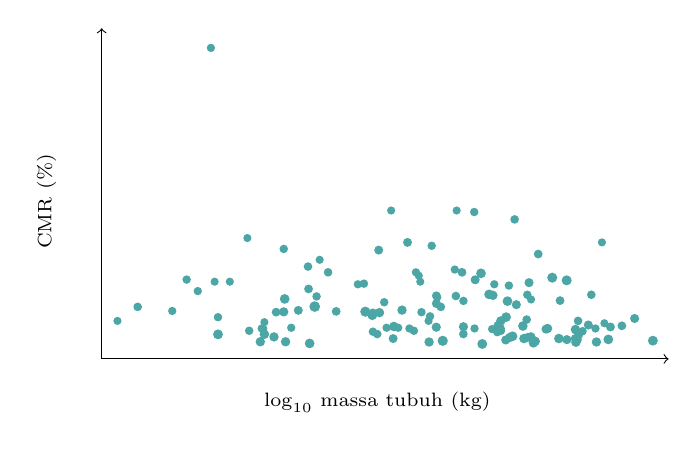
\begin{tikzpicture}[x=1cm,y=1cm]
\draw[->] (0,0) -- (7.2,0);
\draw[->] (0,0) -- (0,4.2);
\node[font=\scriptsize] at (3.5,-0.55) {$\log_{10}$ massa tubuh (kg)};
\node[font=\scriptsize,rotate=90] at (-0.7,2) {CMR (\%)};
\fill[teal!70] (5.057,0.387) circle (0.064);
\fill[teal!70] (5.663,0.387) circle (0.059);
\fill[teal!70] (5.136,0.531) circle (0.062);
\fill[teal!70] (3.814,0.620) circle (0.060);
\fill[teal!70] (5.349,0.418) circle (0.061);
\fill[teal!70] (4.833,0.190) circle (0.063);
\fill[teal!70] (5.070,0.358) circle (0.054);
\fill[teal!70] (3.437,0.556) circle (0.063);
\fill[teal!70] (4.484,1.135) circle (0.053);
\fill[teal!70] (3.991,1.100) circle (0.053);
\fill[teal!70] (5.266,0.689) circle (0.058);
\fill[teal!70] (4.958,0.379) circle (0.053);
\fill[teal!70] (6.768,0.514) circle (0.058);
\fill[teal!70] (6.606,0.421) circle (0.056);
\fill[teal!70] (6.050,0.483) circle (0.055);
\fill[teal!70] (6.271,0.387) circle (0.053);
\fill[teal!70] (2.312,0.598) circle (0.059);
\fill[teal!70] (2.188,0.280) circle (0.060);
\fill[teal!70] (2.066,0.314) circle (0.061);
\fill[teal!70] (2.215,0.594) circle (0.056);
\fill[teal!70] (4.731,1.866) circle (0.054);
\fill[teal!70] (5.131,0.241) circle (0.058);
\fill[teal!70] (5.032,0.427) circle (0.056);
\fill[teal!70] (4.262,0.783) circle (0.052);
\fill[teal!70] (1.477,0.312) circle (0.063);
\fill[teal!70] (4.046,0.981) circle (0.052);
\fill[teal!70] (5.363,0.259) circle (0.061);
\fill[teal!70] (4.743,1.005) circle (0.058);
\fill[teal!70] (4.249,0.403) circle (0.059);
\fill[teal!70] (6.022,0.212) circle (0.060);
\fill[teal!70] (1.850,1.535) circle (0.052);
\fill[teal!70] (1.873,0.358) circle (0.054);
\fill[teal!70] (4.576,1.100) circle (0.056);
\fill[teal!70] (2.729,0.794) circle (0.054);
\fill[teal!70] (5.218,0.288) circle (0.062);
\fill[teal!70] (5.405,0.815) circle (0.054);
\fill[teal!70] (3.444,0.346) circle (0.054);
\fill[teal!70] (1.387,3.950) circle (0.053);
\fill[teal!70] (0.457,0.661) circle (0.055);
\fill[teal!70] (1.477,0.530) circle (0.054);
\fill[teal!70] (6.014,0.259) circle (0.057);
\fill[teal!70] (6.461,0.406) circle (0.057);
\fill[teal!70] (6.107,0.352) circle (0.054);
\fill[teal!70] (6.283,0.215) circle (0.060);
\fill[teal!70] (4.170,0.541) circle (0.054);
\fill[teal!70] (4.594,0.409) circle (0.059);
\fill[teal!70] (3.253,0.948) circle (0.053);
\fill[teal!70] (3.330,0.956) circle (0.054);
\fill[teal!70] (3.499,0.316) circle (0.055);
\fill[teal!70] (4.307,0.661) circle (0.055);
\fill[teal!70] (7.000,0.232) circle (0.063);
\fill[teal!70] (6.040,0.244) circle (0.058);
\fill[teal!70] (5.153,0.734) circle (0.062);
\fill[teal!70] (4.498,0.799) circle (0.055);
\fill[teal!70] (0.896,0.609) circle (0.053);
\fill[teal!70] (5.908,0.245) circle (0.058);
\fill[teal!70] (5.483,0.204) circle (0.061);
\fill[teal!70] (5.427,0.969) circle (0.058);
\fill[teal!70] (0.200,0.483) circle (0.052);
\fill[teal!70] (3.348,0.600) circle (0.065);
\fill[teal!70] (2.497,0.617) circle (0.057);
\fill[teal!70] (4.191,1.437) circle (0.054);
\fill[teal!70] (4.250,0.802) circle (0.056);
\fill[teal!70] (4.735,0.387) circle (0.053);
\fill[teal!70] (4.027,1.057) circle (0.052);
\fill[teal!70] (4.817,1.087) circle (0.062);
\fill[teal!70] (4.594,0.737) circle (0.054);
\fill[teal!70] (3.908,0.387) circle (0.053);
\fill[teal!70] (4.251,0.704) circle (0.058);
\fill[teal!70] (4.061,0.594) circle (0.054);
\fill[teal!70] (4.986,0.948) circle (0.053);
\fill[teal!70] (4.331,0.230) circle (0.065);
\fill[teal!70] (4.920,0.820) circle (0.062);
\fill[teal!70] (3.701,0.259) circle (0.057);
\fill[teal!70] (2.050,0.387) circle (0.053);
\fill[teal!70] (2.066,0.467) circle (0.052);
\fill[teal!70] (1.079,1.008) circle (0.054);
\fill[teal!70] (2.978,0.604) circle (0.056);
\fill[teal!70] (4.158,0.215) circle (0.060);
\fill[teal!70] (2.620,1.173) circle (0.055);
\fill[teal!70] (2.627,0.889) circle (0.056);
\fill[teal!70] (3.765,0.396) circle (0.053);
\fill[teal!70] (5.185,0.274) circle (0.060);
\fill[teal!70] (3.711,0.412) circle (0.061);
\fill[teal!70] (4.508,1.885) circle (0.052);
\fill[teal!70] (2.312,1.397) circle (0.054);
\fill[teal!70] (5.806,0.259) circle (0.061);
\fill[teal!70] (3.588,0.720) circle (0.054);
\fill[teal!70] (3.676,1.885) circle (0.052);
\fill[teal!70] (5.905,0.998) circle (0.064);
\fill[teal!70] (5.244,1.772) circle (0.055);
\fill[teal!70] (5.069,0.483) circle (0.060);
\fill[teal!70] (5.722,1.032) circle (0.064);
\fill[teal!70] (4.968,0.808) circle (0.060);
\fill[teal!70] (4.593,0.316) circle (0.055);
\fill[teal!70] (1.220,0.862) circle (0.053);
\fill[teal!70] (5.544,1.332) circle (0.056);
\fill[teal!70] (5.453,0.755) circle (0.052);
\fill[teal!70] (5.409,0.273) circle (0.057);
\fill[teal!70] (3.618,0.396) circle (0.053);
\fill[teal!70] (4.151,0.483) circle (0.052);
\fill[teal!70] (3.444,0.582) circle (0.059);
\fill[teal!70] (3.884,1.480) circle (0.057);
\fill[teal!70] (2.407,0.396) circle (0.053);
\fill[teal!70] (2.014,0.218) circle (0.060);
\fill[teal!70] (2.768,1.259) circle (0.052);
\fill[teal!70] (5.171,0.932) circle (0.054);
\fill[teal!70] (5.644,0.379) circle (0.059);
\fill[teal!70] (1.434,0.981) circle (0.052);
\fill[teal!70] (5.507,0.224) circle (0.059);
\fill[teal!70] (5.024,0.340) circle (0.054);
\fill[teal!70] (2.335,0.218) circle (0.060);
\fill[teal!70] (2.324,0.762) circle (0.062);
\fill[teal!70] (2.641,0.197) circle (0.062);
\fill[teal!70] (2.032,0.387) circle (0.053);
\fill[teal!70] (3.965,0.358) circle (0.054);
\fill[teal!70] (2.705,0.665) circle (0.068);
\fill[teal!70] (6.353,1.480) circle (0.052);
\fill[teal!70] (6.061,0.308) circle (0.055);
\fill[teal!70] (5.450,0.280) circle (0.060);
\fill[teal!70] (6.180,0.431) circle (0.058);
\fill[teal!70] (5.397,0.500) circle (0.055);
\fill[teal!70] (6.434,0.248) circle (0.062);
\fill[teal!70] (6.017,0.373) circle (0.061);
\fill[teal!70] (1.627,0.981) circle (0.052);
\fill[teal!70] (6.218,0.815) circle (0.055);
\fill[teal!70] (6.384,0.453) circle (0.052);
\fill[teal!70] (3.518,1.382) circle (0.057);
\fill[teal!70] (3.528,0.588) circle (0.060);
\fill[teal!70] (2.875,1.100) circle (0.055);
\fill[teal!70] (5.821,0.741) circle (0.056);
\end{tikzpicture}}
    \caption{Hubungan massa tubuh dan adult cancer mortality risk (CMR).
    Sebaran titik yang lebar menunjukkan bahwa massa tubuh bukan prediktor
    tunggal risiko kanker lintas mamalia.}
    \label{fig:mass-cmr}
\end{figure}

Gambar~\ref{fig:mass-cmr} memperlihatkan pola sebaran tersebut secara visual.
Spesies bermassa besar tidak secara konsisten berada pada CMR tinggi. Hasil ini
tidak berarti massa tubuh melindungi dari kanker, tetapi menunjukkan bahwa
faktor biologis lain perlu dipertimbangkan. Dalam konteks studi ini, faktor
tersebut dieksplorasi melalui simulasi populasi sel.

\subsection{Hasil Simulasi Seluler}

Hasil utama studi ini adalah simulasi berbasis 100 percobaan untuk enam
skenario. Simulasi tidak memprediksi risiko spesies tertentu secara absolut,
tetapi menguji arah perubahan yang termotivasi secara biologis: organisme besar
dan berumur panjang tanpa perlindungan tambahan diperkirakan lebih sering
mengalami cancer escape, sedangkan pembelahan lebih lambat, repair lebih baik,
ambang mutasi lebih tinggi, atau kontrol imun lebih kuat diperkirakan
menurunkan escape probability. Istilah pada tabel perlu dibaca sebagai keluaran
model: escape probability adalah proporsi percobaan berulang yang mengalami
cancer escape sebelum simulasi berakhir, bukan probabilitas kanker nyata pada
spesies tertentu. Mean escape step adalah langkah simulasi pertama saat ambang
imun terlampaui, sedangkan mean final cancer fraction adalah persentase unit
kanker terhadap total unit sel pada akhir simulasi.

% Generated by python main.py via src.simulation_exports.write_simulation_artifacts
% Repeated-trial simulation artifact: n_trials=100, seed=20260528
\begin{table}[t]
\centering
\caption{Ringkasan hasil simulasi seluler untuk skenario Peto's Paradox.}
\label{tab:simulation-summary}
\resizebox{\columnwidth}{!}{%
\begin{tabular}{lrrr}
\toprule
Skenario & Escape probability (\%) & Mean escape step & Mean final cancer fraction (\%)\\
\midrule
Small short-lived & 0.0 & -- & 0.00\\
Large long-lived naive & 72.0 & 384.5 & 0.31\\
Large slower division & 11.0 & 403.8 & 0.03\\
Large better repair & 6.0 & 412.5 & 0.01\\
Large extra required hits & 3.0 & 413.7 & 0.01\\
Large stronger immune control & 0.0 & -- & 0.00\\
\bottomrule
\end{tabular}
}
\end{table}
\newcommand{\SimulationTrialCount}{100}
\newcommand{\SimulationSeed}{20260528}
\newcommand{\SimulationScenarioCount}{6}
\newcommand{\NaiveEscapeProbability}{72.0\%}
\newcommand{\StrongImmuneEscapeProbability}{0.0\%}

Tabel~\ref{tab:simulation-summary} menunjukkan bahwa skenario large long-lived
naive menghasilkan escape probability sebesar \NaiveEscapeProbability{}. Ketika
satu mekanisme protektif diubah, escape probability turun: pembelahan lebih lambat,
repair lebih baik, tambahan required hits, dan kontrol imun lebih kuat semuanya
menurunkan hasil dibanding skenario naive. Pola ini sesuai dengan teori yang
dipakai dalam model. Laju pembelahan dan jumlah hit mengikuti model multi-hit
Caulin dkk. \cite{caulin2015}; repair dan apoptosis mengikuti kerangka
multi-stage cancer progression \cite{szasz2024}; sedangkan cancer escape sebagai
persilangan jumlah sel kanker dengan kapasitas imun mengikuti gagasan tipping
time Kan dan Chen \cite{kan2024}.

Perbedaan antar skenario juga memberi interpretasi biologis yang spesifik.
Pembelahan lebih lambat mengurangi jumlah kesempatan mutasi per waktu hidup,
sehingga sel lebih jarang mencapai ambang transformasi. Repair lebih baik
menurunkan beban mutasi efektif karena sebagian kerusakan kembali diperbaiki
sebelum diwariskan ke pembelahan berikutnya. Tambahan required hits membuat
transformasi kanker membutuhkan lebih banyak kejadian berurutan, sehingga
cancer escape tertunda atau tidak terjadi. Kontrol imun yang lebih kuat tidak
mencegah mutasi awal, tetapi menahan populasi kanker agar tidak melewati
ambang escape. Perbedaan ini penting karena Peto's Paradox kemungkinan tidak
memiliki satu solusi tunggal; beberapa mekanisme dapat bekerja bersama pada
organisme besar atau berumur panjang.

Hasil simulasi dan data empiris saling melengkapi. Data mamalia menunjukkan
bahwa risiko kanker tidak mengikuti skala tubuh secara sederhana, sedangkan
simulasi memperlihatkan mekanisme konseptual yang dapat memutus prediksi naif
tersebut. Dengan demikian, kontribusi utama studi ini adalah model eksploratif
yang dapat direproduksi untuk memahami mengapa organisme besar atau berumur
panjang dapat tetap memiliki risiko kanker yang tidak meningkat secara
proporsional.

\subsection{Eksperimen Simulasi}

Enam skenario pada Tabel~\ref{tab:simulation-summary} dapat dibaca sebagai
eksperimen komputasional kecil. Skenario large long-lived naive berperan sebagai
kontrol naif: jumlah unit sel dan durasi simulasi dibuat lebih besar, tetapi
perlindungan biologis tidak diperkuat. Empat skenario berikutnya mempertahankan
konteks organisme besar dan berumur panjang, lalu mengubah satu mekanisme utama.
Dengan demikian, perbedaan hasil tidak ditafsirkan sebagai perbandingan spesies,
melainkan sebagai perbandingan mekanisme dalam kondisi model yang sama.

Pola hasil memperlihatkan bahwa perlindungan dapat muncul pada tahap berbeda
dari proses kanker. Slower division bekerja di tahap awal karena mengurangi
kesempatan munculnya mutasi baru. Better repair bekerja setelah mutasi muncul,
dengan menurunkan akumulasi kerusakan sebelum sel mencapai status prakanker atau
kanker. Extra required hits mengubah syarat transformasi sehingga kanker
membutuhkan rangkaian kejadian yang lebih panjang. Stronger immune control
bekerja setelah sel kanker muncul, yaitu dengan menahan populasi kanker agar
tidak melewati ambang escape. Karena tiap skenario menekan tahap yang
berbeda, hasil ini mendukung pembacaan bahwa Peto's Paradox tidak harus
dijelaskan oleh satu mekanisme tunggal.

Meskipun skenario dalam eksperimen ini diuji secara terpisah untuk mengisolasi
efek masing-masing mekanisme, dalam biologi nyata mekanisme protektif tersebut
dapat bekerja secara kolektif dan bersinergi. Di bawah kerangka model teoretis
Caulin dkk. \cite{caulin2015}, efek dari intervensi ganda bersifat multiplikatif:
jika laju pembelahan sel normal diturunkan bersamaan dengan efisiensi perbaikan
DNA yang lebih tinggi, laju akumulasi mutasi akan ditekan secara eksponensial
jauh sebelum sel mencapai ambang transformasi. Hal ini menjelaskan mengapa
organisme dengan ukuran tubuh ribuan kali lebih besar tidak memerlukan peningkatan
perlindungan linier sebesar ribuan kali lipat; kombinasi sinergis dari beberapa
perubahan kecil pada parameter seluler sudah cukup untuk memutus hubungan antara
jumlah sel dan risiko kanker.

Nilai probabilitas pada tabel juga perlu dibaca sebagai ukuran relatif dalam
eksperimen simulasi. Angka 72{,}0\% pada skenario organisme besar tanpa
kompensasi biologis berarti 72 dari 100
percobaan stokastik mengalami cancer escape di bawah parameter tersebut. Angka
itu bukan estimasi kejadian kanker pada hewan besar di dunia nyata. Kegunaannya
terletak pada kontras: ketika satu mekanisme protektif dimasukkan, fraksi
percobaan yang mengalami cancer escape turun. Kontras inilah yang menjadi
inti eksperimen, karena menunjukkan bagaimana perubahan proses seluler atau
imun dapat memutus prediksi naif bahwa organisme besar dan panjang umur harus
selalu memiliki risiko kanker jauh lebih tinggi.

\subsection{Keterbatasan}

Model memakai unit sel yang diskalakan, bukan sel biologis individual. Model
belum memuat struktur spasial jaringan, angiogenesis, metabolisme, game theory
penuh, atau parameter spesifik per spesies. Dataset empiris juga berasal dari
mamalia di bawah perawatan manusia dan belum dikontrol secara filogenetik.
Karena itu, hasil tidak boleh dibaca sebagai prediksi risiko kanker nyata atau
bukti bahwa satu mekanisme tertentu bekerja pada spesies tertentu.

Pengembangan berikutnya adalah menghubungkan simulasi dengan estimasi jumlah
sel, laju pembelahan per jaringan, data genomik, dan kontrol filogenetik.
Namun, untuk laporan ringkas ini, enam skenario utama dipilih agar hubungan
antara teori, parameter, dan hasil tetap jelas.
